%
% $RCSfile: method.tex,v $
%
% Copyright (C) 2002-2008. Christian Heller.
%
% Permission is granted to copy, distribute and/or modify this document
% under the terms of the GNU Free Documentation License, Version 1.1 or
% any later version published by the Free Software Foundation; with no
% Invariant Sections, with no Front-Cover Texts and with no Back-Cover
% Texts. A copy of the license is included in the section entitled
% "GNU Free Documentation License".
%
% http://www.cybop.net
% - Cybernetics Oriented Programming -
%
% http://www.resmedicinae.org
% - Information in Medicine -
%
% Version: $Revision: 1.1 $ $Date: 2008-08-19 20:41:07 $ $Author: christian $
% Authors: Christian Heller <christian.heller@tuxtax.de>
%

\section{Method}
\label{method_heading}
\index{Method}
\index{Traditional and New Ideas}
\index{Merger of traditional and new Concepts}
\index{Statics and Dynamics}
\index{Knowledge Schema}
\index{State and Logic}

Despite all scientific methodology, research is mostly a journey into the blue.
Likewise did this work not follow a linear way of progression, but rather a
zigzag course between theory and practice (figure \ref{constructive_figure}),
which may be labelled \emph{Constructive Development}.

\begin{figure}[ht]
    \begin{center}
        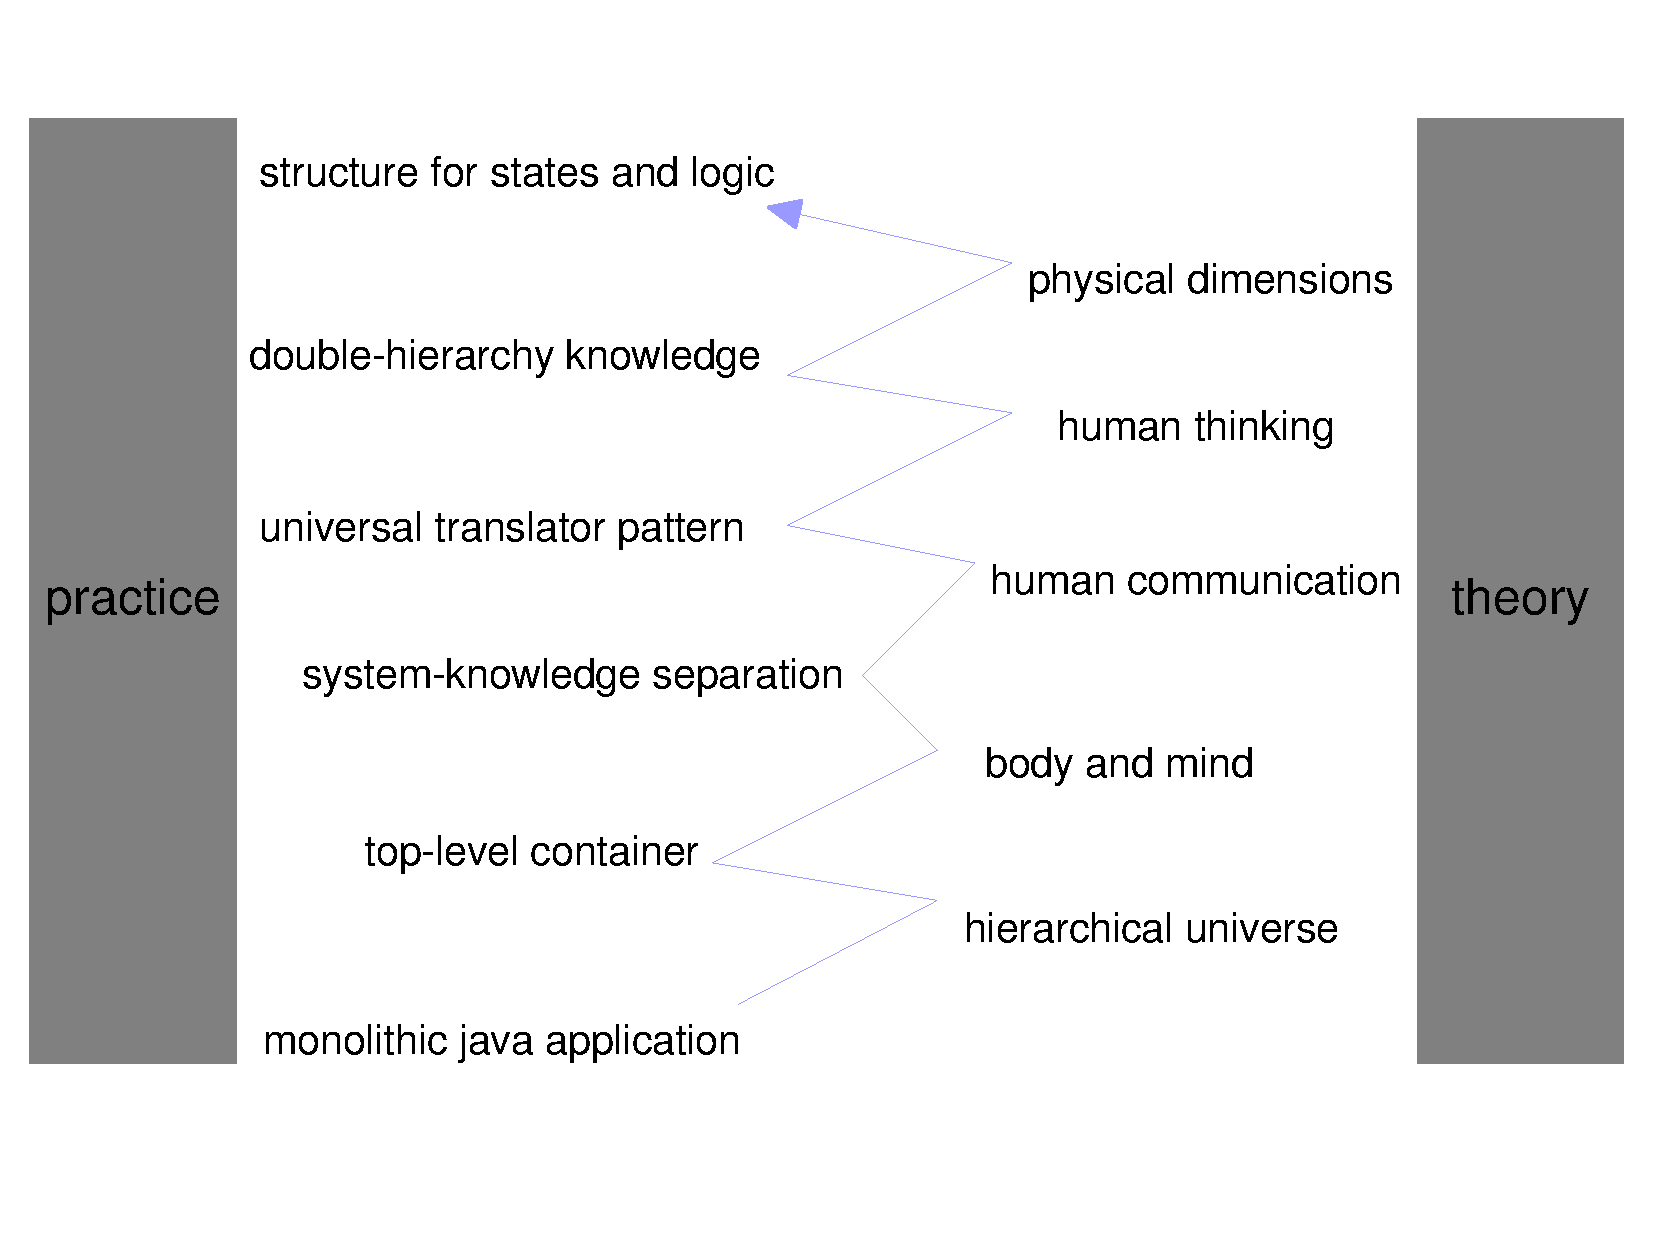
\includegraphics[scale=0.3,angle=-90]{graphic/constructive.pdf}
        \caption{Constructive Development}
        \label{constructive_figure}
    \end{center}
\end{figure}

At the beginning, there was the wish to create a software application for use
in medicine. Development started off by using classical programming techniques.
Whenever a problem occured, it was solved by applying yet more up-to-date
techniques and latest software design principles, such as \emph{Patterns}. This
worked out well until the point at which the complexity of the software could
not be handled easily anymore and new ideas were demanded.

It was only when state-of-the-art concepts got more and more unsatisfying and
insufficient to maintain a clear architecture, that new ones had to be found.
After some time of reflexion, the principles of human thinking for abstracting
the real world in artificial models could be identified as source of new ideas
for software design. Further ideas were later taken over from other phenomenons
of nature and various scientific disciplines. The obvious similarities between
human- and computer systems (information input, -storage, -processing, -output)
should be rationale enough for an inter-disciplinary approach.

\begin{figure}[ht]
    \begin{center}
        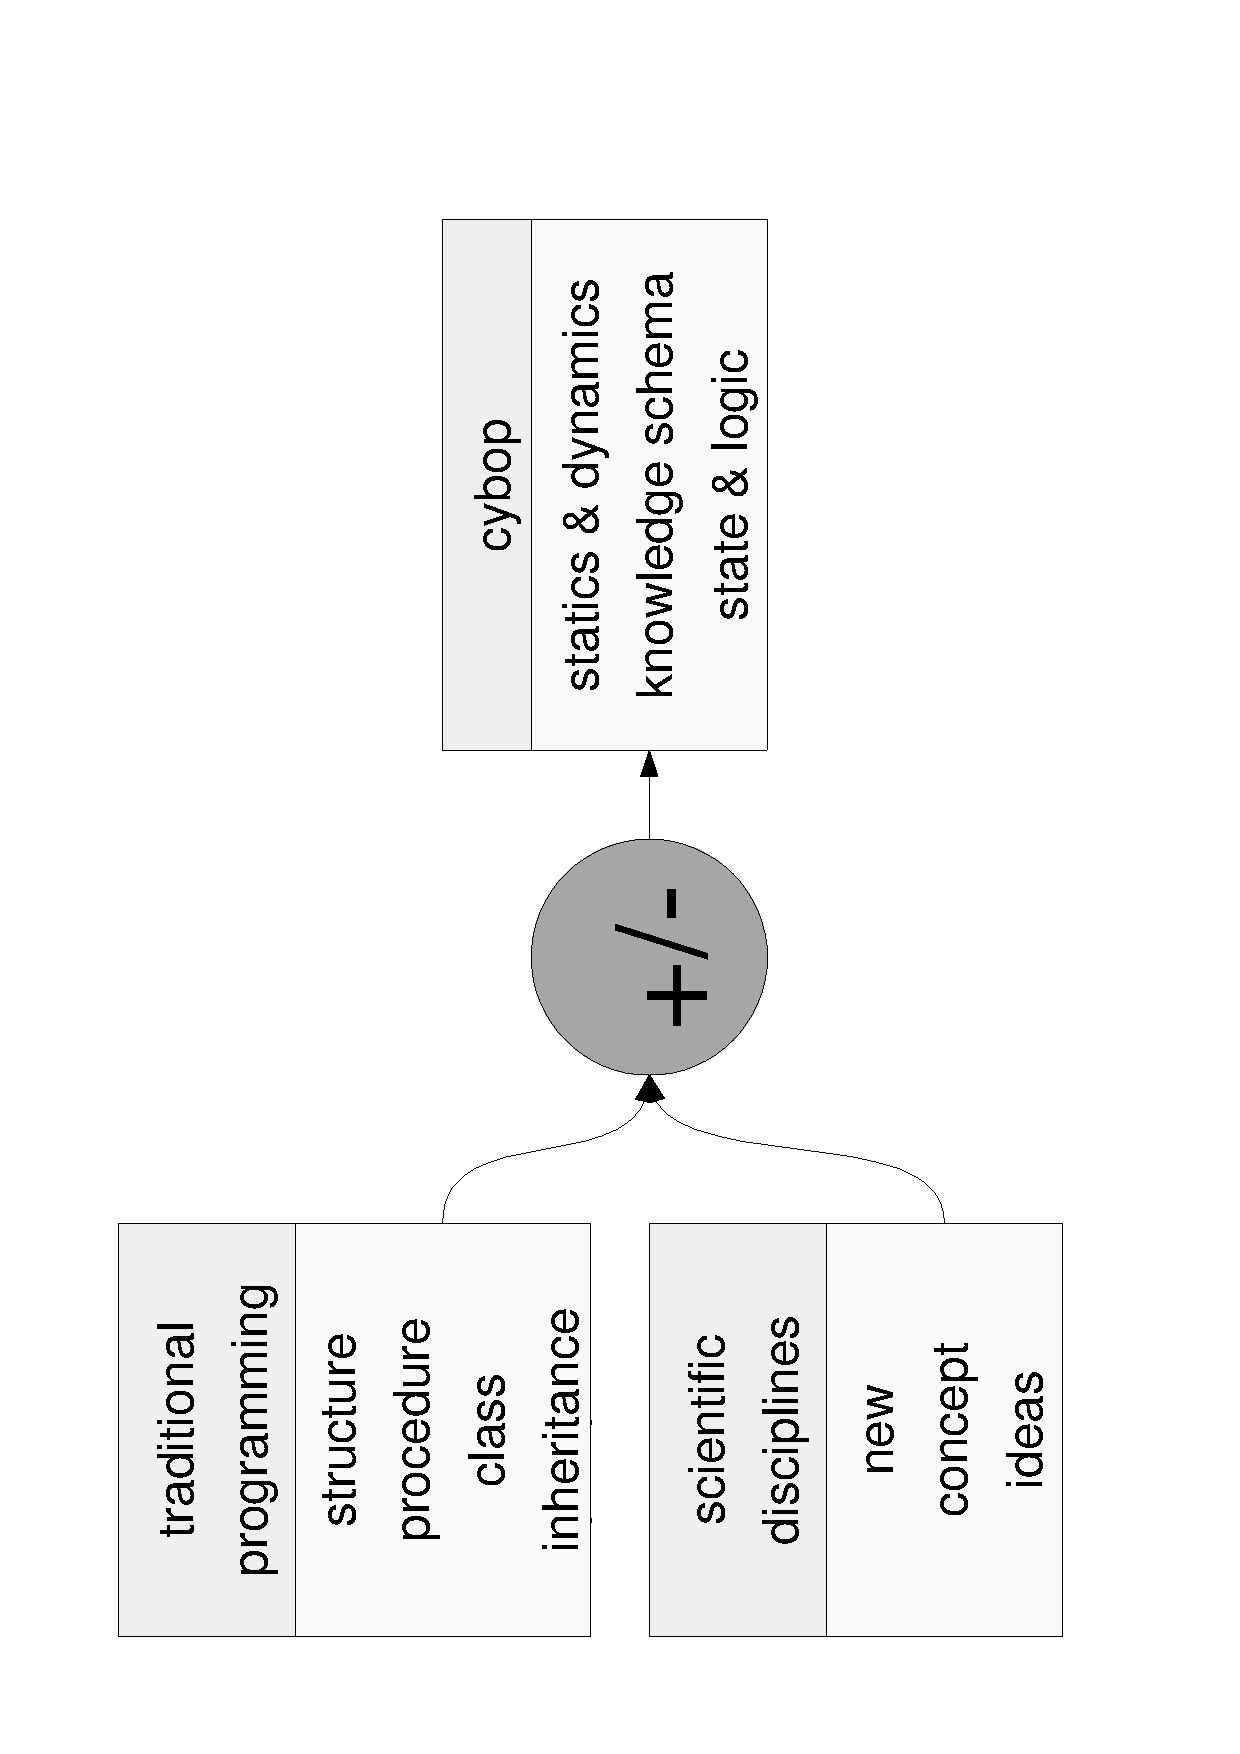
\includegraphics[scale=0.3,angle=-90]{graphic/method.pdf}
        \caption{Merger of traditional and new Concepts}
        \label{method_figure}
    \end{center}
\end{figure}

The concepts resulting from both, traditional and new ideas, got finally merged
and developed towards the CYBOP theory (figure \ref{method_figure}). For this
new kind of programming, the distinction of \emph{Statics and Dynamics}, a
special \emph{Knowledge Schema} and the separation of \emph{State and Logic}
are necessary. Chapter \ref{extended_motivation_heading} will define these in
greater detail.

This work reports about the progress of finding new ideas for software design.
However, since problems did not occur in a predictable way, while developing
the mentioned application, their presentation in order of appearance would be
rather confusing. A systematised structure of sections is therefore used in
this work to organise most problems after the programming paradigm they belong
to. For the interested reader, chapter \ref{res_medicinae_heading} describes
the stepwise construction and taken design decisions of the prototype anyway.
